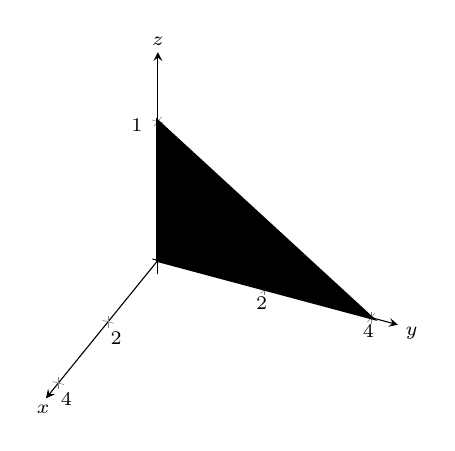
\begin{tikzpicture}[>=stealth]
\begin{axis}%
[width=175pt,height=200pt,
tick label style={font=\scriptsize},%axis on top,
			axis lines=center,
			view={115}{35},
			name=myplot,
			%xtick={1,2,3,4},
			%ytick={1,2,3,4,5,6},
			%ztick=\empty,
			%extra x ticks={1},
			%minor x tick num=1,
			%minor y tick num=4,
			%minor z tick num=1,
			%extra x tick labels={$a$},
			%extra y ticks={1},
			%extra y tick labels={$a$},
			%extra z ticks={1},
			%extra z tick labels={$h$},
			ymin=-.1,ymax=4.5,
			xmin=-.1,xmax=4.5,
			zmin=-.1, zmax=1.5,
			every axis x label/.style={at={(axis cs:\pgfkeysvalueof{/pgfplots/xmax},0,0)},xshift=-1pt,yshift=-4pt},
				xlabel={\scriptsize $x$},
			every axis y label/.style={at={(axis cs:0,\pgfkeysvalueof{/pgfplots/ymax},0)},xshift=5pt,yshift=-3pt},
				ylabel={\scriptsize $y$},
				every axis z label/.style={at={(axis cs:0,0,\pgfkeysvalueof{/pgfplots/zmax})},xshift=0pt,yshift=4pt},
				zlabel={\scriptsize $z$}
			]


%\draw [{\colortwo},thick] (axis cs: 0,4,0) -- (axis cs: 2,4,-6) -- (axis cs: 2,0,2);

\draw [very thick,{\colorone},fill={\coloronefill}] (axis cs:0,0,0) -- (axis cs:0,4,0)-- (axis cs:0,0,1)--cycle;

%\addplot3[domain=0:2,,y domain=0:1,surf,%fill=white,
%colormap={mp2}{\colormapplaneone},opacity=.8,faceted color=black!40,samples=9,samples y=4,very thin,z buffer=sort] ({x},{y*(4-2*x)+2*x},{1-(y*(4-2*x)+2*x)/4});
%
%\addplot3[domain=0:2,,y domain=0:1,surf,%fill=white,
%colormap={mp2}{\colormapplaneone},opacity=.8,faceted color=black!40,samples=9,samples y=4,very thin,z buffer=sort] ({x},{y*(2*x)},{1-x/2});
%
%\draw [{\colorone},very thick] (axis cs: 0,0,1) -- (axis cs: 2,0,0) -- (axis cs: 2,4,0)-- cycle
															%(axis cs:0,0,1) -- (axis cs: 0,4,0) -- (axis cs:2,4,0);
%
%\draw [->] (axis cs:3,2,0) node[below,rotate=-15] {\scriptsize $z=1-\frac12x$} -- (axis cs: 1.5,2,0);
%
%\draw [->] (axis cs:0,2.5,.6) node[above,rotate=-30] {\scriptsize $z=1-\frac14y$} -- (axis cs: .25,3,0);

%\draw [->] (axis cs:0,-.4,1.2) node[above,] {\scriptsize $z=-y$} -- (axis cs: 0,-.4,.6);
%\draw [{\colorone}, very thick] (axis cs:0,0,0) -- (axis cs:0,0,2)
																		%(axis cs:0,0,0) -- (axis cs:3,0,0)
																		%(axis cs:0,0,0) -- (axis cs:0,6,0);
		%


\end{axis}


\end{tikzpicture}












